\normalfalse \difficilefalse \tdifficiletrue
\correctionfalse

%\UPSTIidClasse{11} % 11 sup, 12 spé
%\newcommand{\UPSTIidClasse}{12}

\exer{Système 4 barres $\star\star\star$ \label{CIN:02:B2:13:17}} 
\setcounter{question}{0}\marginnote{\xpComp{CIN}{02}}%\UPSTIcompetence[2]{B2-13}
\index{Compétence B2-13}\index{Compétence CIN-02}
\index{Système 4 barres}
\ifcorrection
\else
\marginnote{\textbf{Pas de corrigé pour cet exercice.}}
\fi

\ifprof
\else
On a : 
%\begin{multicols}{2}
\begin{itemize}
\item $\vect{OA} = a \vx{1}-f \vy{1}$ avec $a=\SI{355}{mm}$ et $f=\SI{13}{mm}$;
\item $\vect{AB} = b \vx{2}$ avec $b=\SI{280}{mm}$;
\item $\vect{BC} = -c \vx{3}$ avec $c=\SI{280}{mm}$;
\item $\vect{OC} = -d \vx{0}-e\vy{0}$ avec $d=\SI{89,5}{mm}$ et $e=\SI{160}{mm}$;
\end{itemize}
%\end{multicols}
%a,b,c,d,e,ff = 355,280,280,89.5,160,13

\begin{marginfigure}
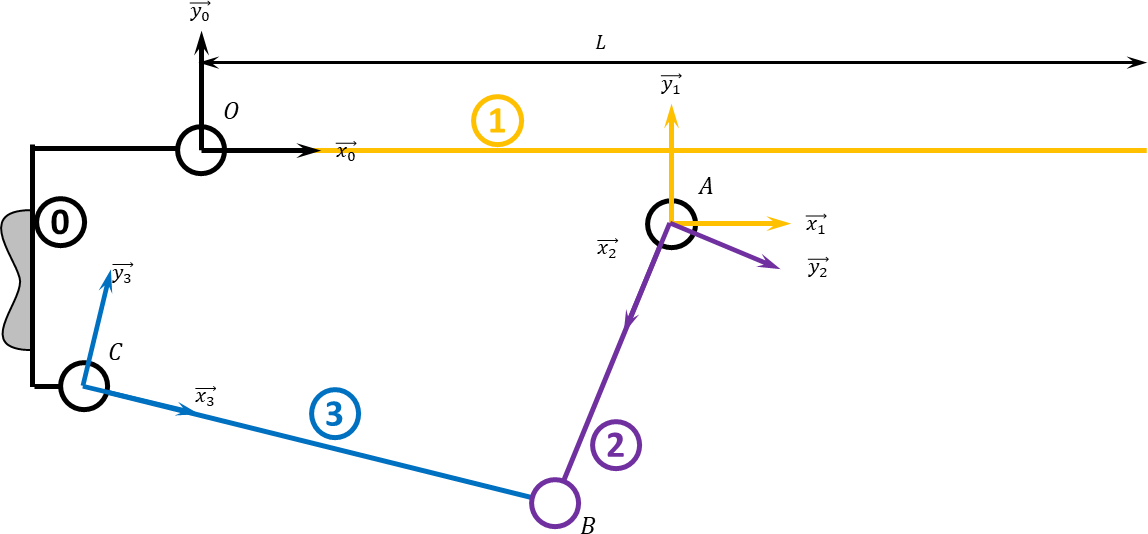
\includegraphics[width=\linewidth]{17_01}

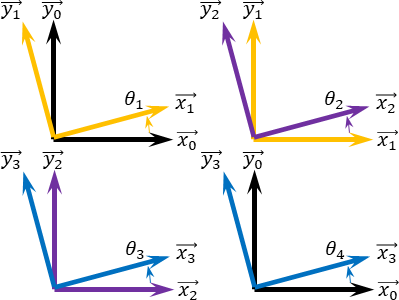
\includegraphics[width=\linewidth]{17_02}
\end{marginfigure}
\fi
Il est possible de mettre la loi entrée-sortie sous la forme *** (voir exercice \ref{C2:06:17}).
On définit le point $G$ tel que $\vect{OG}=L\vect{x_1}$.

\question{Donner le torseur cinématique $\torseurcin{V}{1}{0}$ au point $G$.}
\ifprof
\else
\fi

\question{Déterminer $\vectg{G}{1}{0}$.}
\ifprof
\else
\fi

\ifprof
\else
\begin{flushright}
\footnotesize{Corrigé  voir \ref{CIN:02:B2:13:17}.}
\end{flushright}%
\fi